\documentclass[aspectratio=169,11pt,serif,professionalfonts]{beamer}
%\documentclass[11pt,serif,professionalfonts]{beamer}
\mode<presentation>
%%\usepackage[utf8]{inputenc}
%\usepackage[T1]{fontenc}
\usepackage{fancybox}
\usepackage{macros/themes/darktheme}
\usepackage{amssymb}
\usepackage{amsmath}
\usepackage{booktabs}
\usepackage{esint}
\usepackage{multicol}
\usepackage{textcomp}
\usepackage{animate}
\usepackage[printwatermark]{xwatermark}
%\newwatermark*[pages=1,angle=0,scale=.35,xpos=-60,ypos=-20]{
\includegraphics[height=1\paperheight]{macros/logo/armesclair.pdf}}
%\newwatermark*[pages=1,angle=0,scale=.28,xpos=55,ypos=33]{
\includegraphics[height=0.8\paperheight]{macros/logo/logo_purple.png}}
\graphicspath{{img/}}
\usepackage{soul}
\usepackage{animate}
%\usepackage{CJKutf8}
%\usepackage{pbsi}
\usepackage{tcolorbox}
%\usepackage[english,japanese]{babel}
\usefonttheme{professionalfonts}
\usepackage{tikz}
\usetikzlibrary{arrows,shapes,backgrounds}
\usepackage{physics}
\usepackage{soul}
\usepackage{xeCJK}
\setCJKmainfont{AozoraMinchoRegular.ttf}
\usepackage{empheq}
\usepackage[T1]{fontenc}
\usepackage{concmath}
\makeatletter
\newcommand\Cshadowbox{\VerbBox\@Cshadowbox}
\def\@Cshadowbox#1{%
  \setbox\@fancybox\hbox{\fbox{#1}}%
  \leavevmode\vbox{%
    \offinterlineskip
    \dimen@=\shadowsize
    \advance\dimen@ .5\fboxrule
    \hbox{\copy\@fancybox\kern.5\fboxrule\lower\shadowsize\hbox{%
      \color{ultralightbleu303}\vrule \@height\ht\@fancybox \@depth\dp\@fancybox \@width\dimen@}}%
    \vskip\dimexpr-\dimen@+0.5\fboxrule\relax
    \moveright\shadowsize\vbox{%
      \color{ultralightbleu303}\hrule \@width\wd\@fancybox \@height\dimen@}}}
\makeatother

\def\Put(#1,#2)#3{\leavevmode\makebox(0,0){\put(#1,#2){#3}}}
\definecolor{bleu303}{RGB}{0,90,135}
\definecolor{bg}{HTML}{00FFFF}
\renewcommand{\d}{{d}}


\setbeamertemplate{frametitle}[default][center]
\addtobeamertemplate{frametitle}{\vspace{-.5\baselineskip}}


\definecolor{rouge}{RGB}{213,43,30}             
\definecolor{vert575}{HTML}{00C41A}             
\colorlet{vert}{black!20!vert575}           



\AtBeginSection[]
  {
    \ifnum \value{framenumber}>5
    \begin{frame}<beamer>\frametitle{\underline{Outline}}
\begin{minipage}{.1\linewidth}\hfill\vfill\end{minipage}\begin{minipage}{.8\linewidth}\tableofcontents[currentsection] \end{minipage}
\end{frame}
    \else
    \fi
  }
\AtBeginSection[]{\stepcounter{subsection}}


\usepackage{fancybox}
\usepackage{macros/themes/whitetheme}
\usepackage{amssymb}
\usepackage{amsmath}
\usepackage{booktabs}
\usepackage{esint}
\usepackage{multicol}
\usepackage{textcomp}
\usepackage{animate}
\usepackage[printwatermark]{xwatermark}
%\newwatermark[pages=1,angle=0,scale=1,xpos=0,ypos=0]{
\includegraphics[height=0.8\paperheight]{macros/taplogo.eps}}
\graphicspath{{img/}}
\usepackage{soul}
\usepackage{animate}
%\usepackage{CJKutf8}
\usepackage{pbsi}
\usepackage{tcolorbox}
%\usepackage[english,japanese]{babel}
%\usefonttheme{serif}
\usefonttheme{professionalfonts}
\usepackage{tikz}
\usetikzlibrary{arrows,shapes,backgrounds}
\usepackage{physics}
\usepackage{xeCJK}
\setCJKmainfont{AozoraMinchoRegular.ttf}
\usepackage{empheq}
\usepackage[T1]{fontenc}
\usepackage{concmath}
\makeatletter
\newcommand\Cshadowbox{\VerbBox\@Cshadowbox}
\def\@Cshadowbox#1{%
  \setbox\@fancybox\hbox{\fbox{#1}}%
  \leavevmode\vbox{%
    \offinterlineskip
    \dimen@=\shadowsize
    \advance\dimen@ .5\fboxrule
    \hbox{\copy\@fancybox\kern.5\fboxrule\lower\shadowsize\hbox{%
      \color{darkbleu303}\vrule \@height\ht\@fancybox \@depth\dp\@fancybox \@width\dimen@}}%
    \vskip\dimexpr-\dimen@+0.5\fboxrule\relax
    \moveright\shadowsize\vbox{%
      \color{darkbleu303}\hrule \@width\wd\@fancybox \@height\dimen@}}}
\makeatother

\def\Put(#1,#2)#3{\leavevmode\makebox(0,0){\put(#1,#2){#3}}}
\definecolor{bleu303}{RGB}{0,90,135}
\definecolor{bg}{HTML}{00FFFF}
\renewcommand{\d}{{d}}

%\usepackage{textpos}

\setbeamertemplate{frametitle}[default][left]
\addtobeamertemplate{frametitle}{\vspace{-.3\baselineskip}}
%\addtobeamertemplate{frametitle}{}{%
%\begin{textblock*}{100mm}(.85\textwidth,-.5cm)
%
\includegraphics[height=1.5cm,keepaspectratio]{macros/taplogof.eps}
%\end{textblock*}}

\definecolor{rouge}{RGB}{213,43,30}             
\definecolor{vert575}{HTML}{00C41A}             
\colorlet{vert}{black!20!vert575}           

\tikzstyle{every picture}+=[remember picture]
\tikzstyle{na} = [baseline=-.5ex]
\everymath{\displaystyle}


\AtBeginSection[]
  {
    \ifnum \value{framenumber}>5
      \begin{frame}<beamer>
      \frametitle{Plan}
      \tableofcontents[currentsection]
      \end{frame}
    \else
    \fi
  }

\AtBeginSection[]{\stepcounter{subsection}}




\title{A shorter way of writing the title}
\author{Pierre~Goux} 
\date{lieu ou \today}

\setbeamersize{text margin left=7mm,text margin right=7mm} 

\hypersetup{pdfstartview={Fit}} 
%\addtobeamertemplate{background canvas}{}{\transfade[duration=0.1]}

\begin{document}
%\begin{frame}{\underline{\small{}}}
\vspace{-.5em}
\begin{center}
\boxput*(0,1){
    \colorbox{black}{\textcolor{ultralightbleu303}{\large{\textit{Short Surtitle}}}}
}{    
\setlength{\fboxsep}{5pt}
\Cshadowbox{\begin{minipage}{.7\linewidth}
\vspace{.25em}
\begin{small}
\centering
\textcolor{ultralightbleu303}{\LARGE{\textbf{Pourquoi c'est vide}}\\
\vspace{.2em}
\LARGE{\textbf{Title of the very interesting stuff と日本語版への翻訳}}}\\
\vspace{.5em}
\end{small}
\end{minipage}}
}\\
\vspace*{2em}
\centering
Pierre \textsc{Goux}$^1$, Mars 20, 2018 \\
\vspace{1.5em}

\begin{minipage}{.2\linewidth}\hfill\vfill\end{minipage}\begin{minipage}{.75\linewidth}\textit{\small{Outline of the stuff, commentary, abstract, or whatever seems useful to be put there } }\end{minipage}
\end{center}
\vspace{.5em}
\begin{flushright}
\footnotesize $^1$ Ecole polytechnique, CNRS, affiliation
\end{flushright}

\end{frame}
%
%\setbeamertemplate{background canvas}{%
%    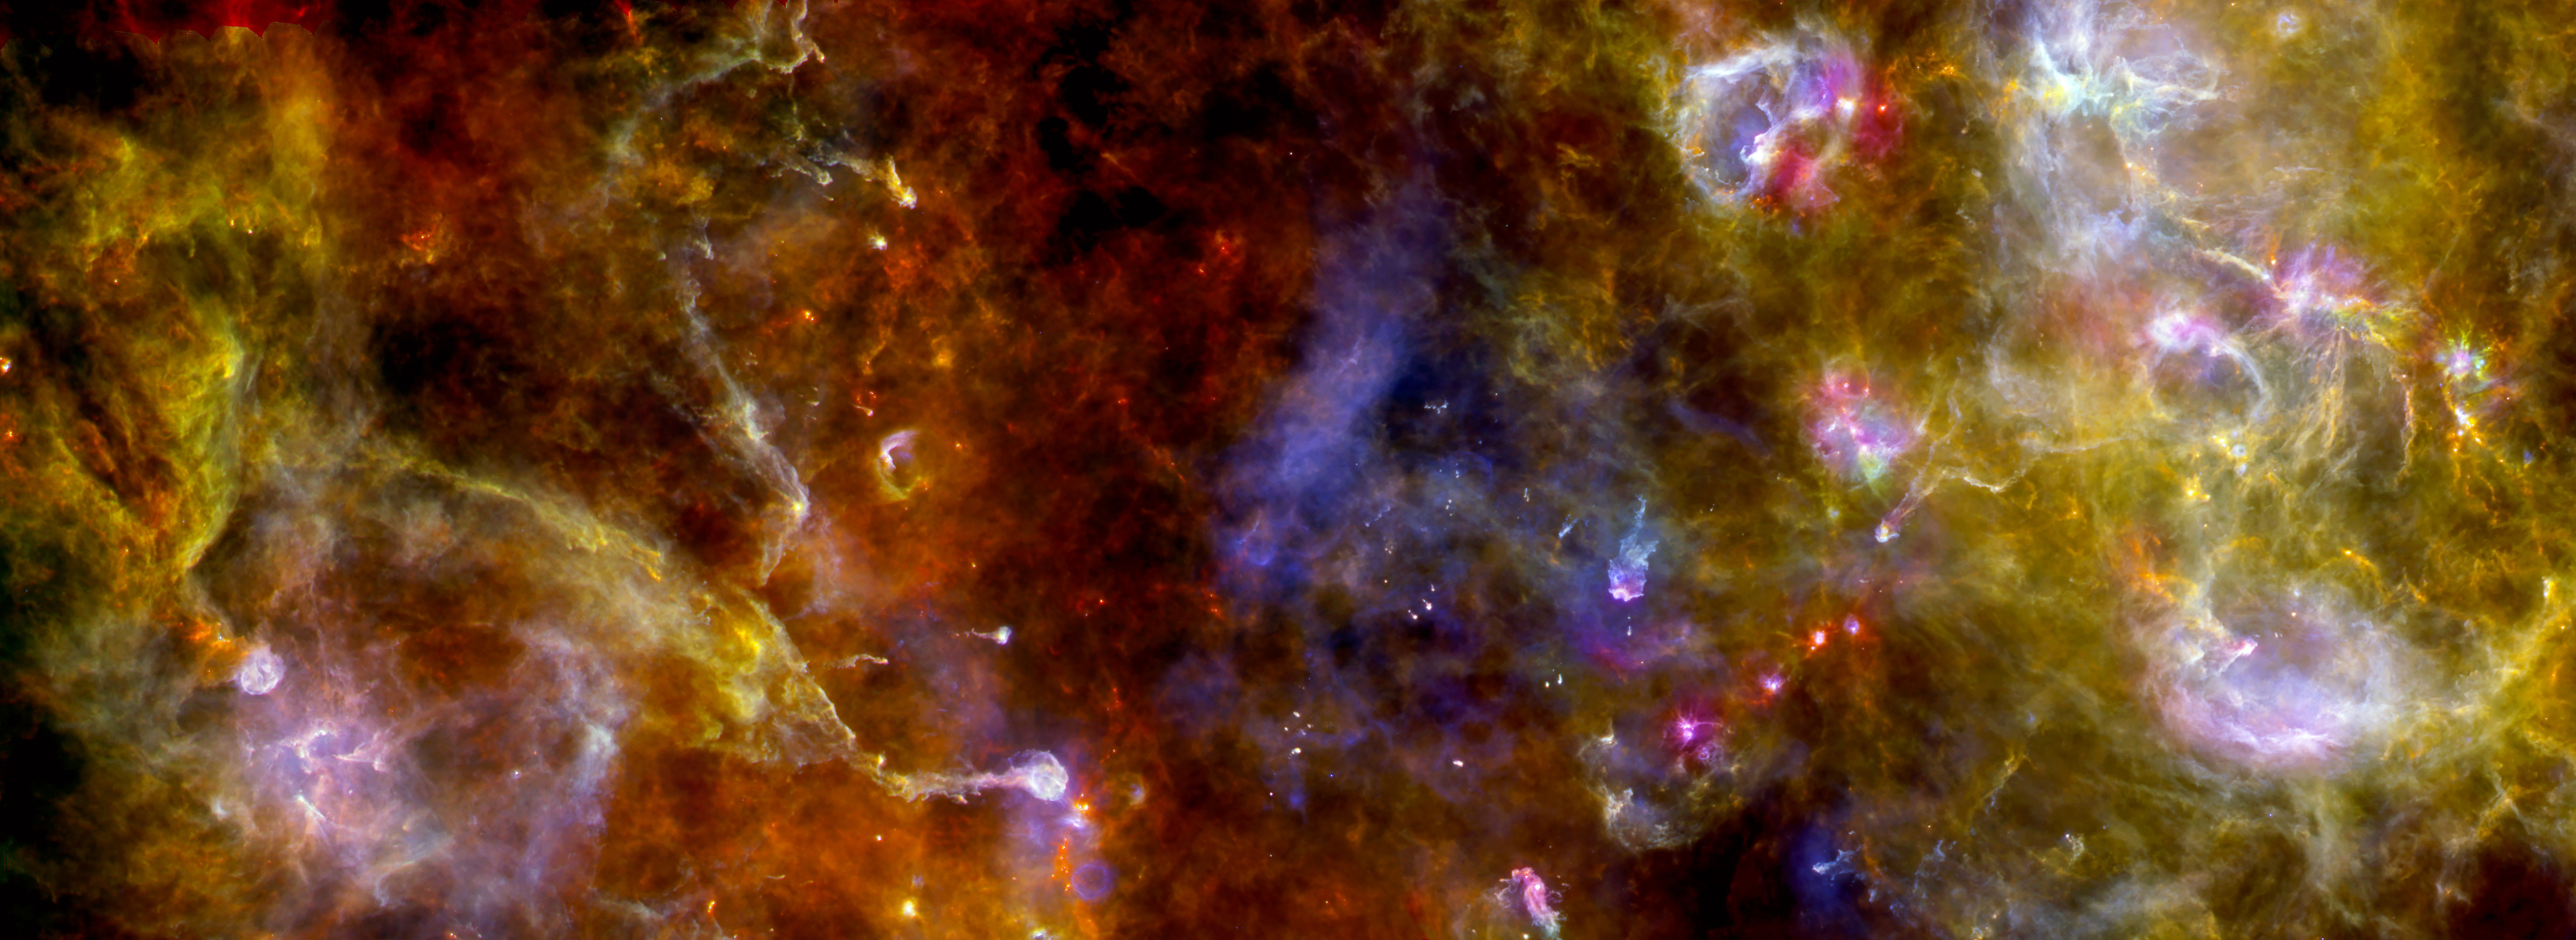
\includegraphics[width=\paperwidth,height=\paperheight]{img/Herschel_s_swan.jpg}
%}

\begin{frame}[plain]{}
\centering
\vspace{\baselineskip}
\begin{center}
\boxput*(0,1){
    \colorbox{black}{\textcolor{yellow!05}{日本物理学会2018年秋季大会
}}
}{    
\setlength{\fboxsep}{5pt}
\Cshadowbox{\begin{minipage}{.85\linewidth}
\vspace{.75em}
\begin{small}
\centering
\textcolor{yellow!05}{\LARGE{\textbf{\sffamily Structures of the cold neutral medium}}\\
\vspace{.5em}
%\Large{\textbf{ \sffamily from thermal neutron capture on Gadolinium}}
}   
\vspace{.5em}
\end{small}
\end{minipage}}
}\\
\vspace{.7\baselineskip}
\begin{minipage}{.85\linewidth}\centering\large \color{yellow!05} 濃縮ガドリニウム($^{\mathbf{155,157}}$Gd)の熱中性子捕獲反応から放出される離散的及び連続的遷移のガンマ線間の角度相関について\\\end{minipage}
\end{center}
\vspace{\baselineskip}
\begin{columns}
\begin{column}[T]{.3\linewidth}
\centering
%
\includegraphics[width=.5\linewidth]{macros/logo/polytechnique-logohori.pdf}
\end{column}
\begin{column}[T]{.4\linewidth}\vspace{-\baselineskip}
\begin{center}\large{Pierre \textsc{Goux}}$\color{yellow!05}\mathbf{^{2,1}}$\\ \vspace{.5em}{平成30年9月14日} \\
\end{center}
\end{column}        
\begin{column}[T]{.3\linewidth}
%\centering\includegraphics[width=.5\linewidth]{macros/logo/annrigd.png}
\end{column}
\end{columns}\vspace{\baselineskip}
\begin{minipage}{.92\linewidth}
田中智之$\color{yellow!05}\mathbf{^1}$, 須藤高志$\color{yellow!05}\mathbf{^1}$, A. \textsc{Ajmi}$\color{yellow!05}\mathbf{^1}$, 
\end{minipage}
\vspace{.6em}

\footnotesize{\textit{$\color{yellow!05}\mathbf{^1}$Okayama University, $\color{yellow!05}\mathbf{^2}$ Ecole polytechnique} 
}
\vspace{\baselineskip}
\end{frame}

\setbeamertemplate{background canvas}{%
    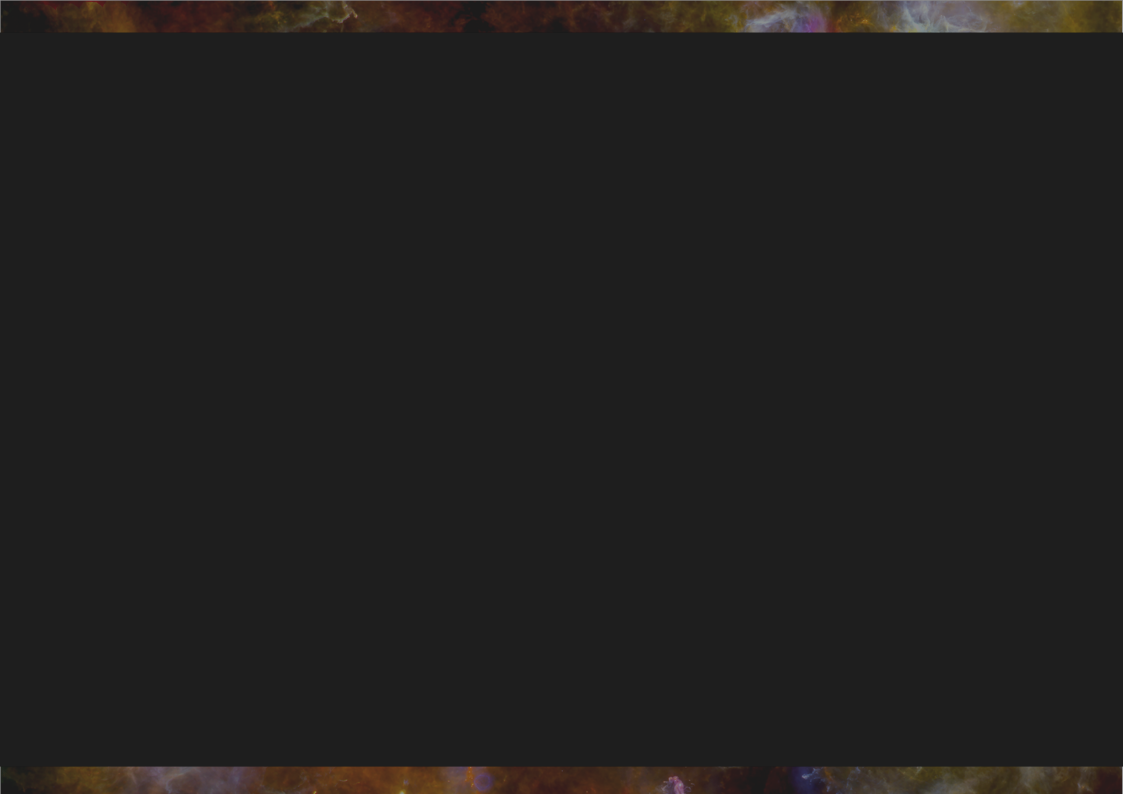
\includegraphics[width=\paperwidth,height=\paperheight]{macros/drawing.png}
}
%\newcommand\AtPagemyLowerRight[1]{\AtPageLowerLeft{%
%\put(\LenToUnit{0.02\paperwidth},\LenToUnit{0.89\paperheight}){#1}}}
%\AddToShipoutPictureFG{
%  \AtPagemyLowerRight{{
\includegraphics[width=2cm,keepaspectratio]{macros/logo/polytechnique-logohori.pdf}}}
%}%


\setbeamertemplate{background canvas}{%
    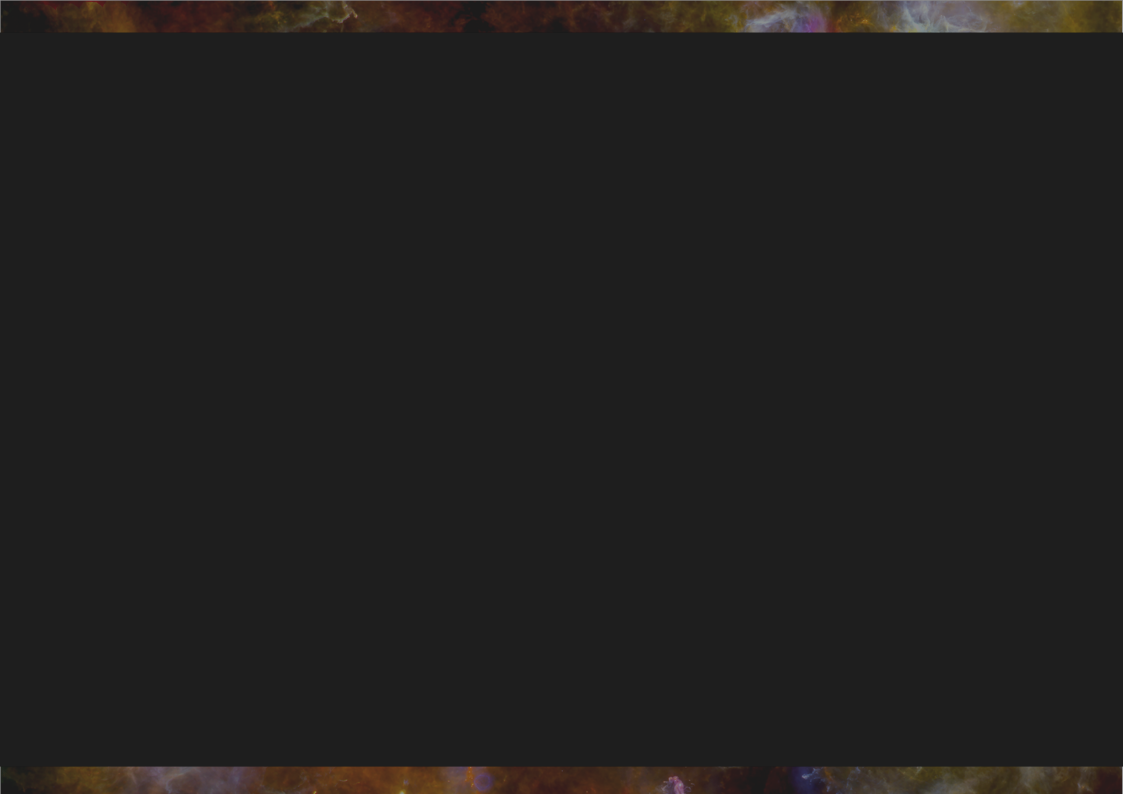
\includegraphics[width=\paperwidth,height=\paperheight]{macros/drawing.png}
}

\begin{frame}[plain]
\begin{center}
\boxput*(0,1){
    \colorbox{white}{\textcolor{darkbleu303}{\large{\textit{Short Surtitle}}}}
}{    
\setlength{\fboxsep}{5pt}
\Cshadowbox{\begin{minipage}{.7\linewidth}
\vspace{.5em}
\begin{small}
\centering
\textcolor{darkbleu303}{\Large{\textbf{Pourquoi c'est vide}}\\
\vspace{.2em}
\Large{\textbf{Title of the interesting stuff}}}\\
\vspace{.5em}
\end{small}
\end{minipage}}
}\\
\vspace*{.5em}
\centering
{\large{\textbf{日本語でも書くことができる\\\vspace{.5em}
\textcolor{bleu303}{難しい漢字も憂鬱とか鬮とか瘠とか薔薇}}}}\\
\vspace*{1.5em}
Pierre \textsc{Goux}$^1$,  \\
\vspace{1em}
    
\textit{\small{Outline of the stuff, commentary, abstract, or whatever seems useful to be put there } }
\end{center}
\vspace{.5em}
\begin{flushright}
\footnotesize $^1$ Ecole polytechnique, CNRS, affiliation
\end{flushright}
\small{\today}
\end{frame}

%\newcommand\AtPagemyLowerRight[1]{\AtPageLowerLeft{%
%\put(\LenToUnit{0.05\paperwidth},\LenToUnit{0.84\paperheight}){#1}}}
%\AddToShipoutPictureFG{
%  \AtPagemyLowerRight{{
\includegraphics[width=1cm,keepaspectratio]{macros/logo/armes.pdf}}}
%}%
\setbeamertemplate{background canvas}{%
    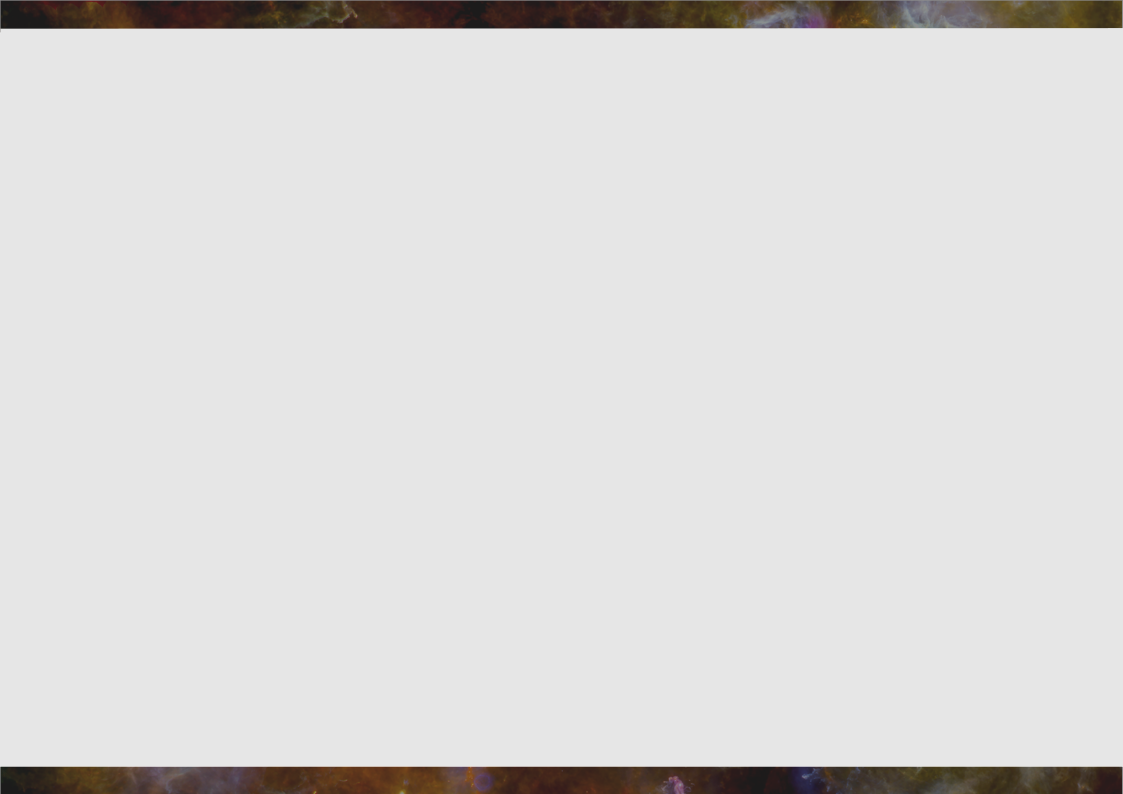
\includegraphics[width=\paperwidth,height=\paperheight]{macros/drawing3.png}
}

%\begin{frame}[plain]{}
\begin{center}
\boxput*(0,1){
    \colorbox{white}{\textcolor{bleu303}{\large{\textit{Short Surtitle}}}}
}{    
\setlength{\fboxsep}{5pt}
\Cshadowbox{\begin{minipage}{.7\linewidth}
\vspace{.5em}
\begin{small}
\centering
\textcolor{bleu303}{\Large{\textbf{Pourquoi c'est vide}}\\
\vspace{.2em}
\Large{\textbf{Title of the interesting stuff}}}\\
\vspace{.5em}
\end{small}
\end{minipage}}
}\\
\vspace*{.5em}
\centering
{\large{\textbf{日本語でも書くことができる\\\vspace{.5em}
\textcolor{bleu303}{難しい漢字も憂鬱とか鬮とか瘠とか薔薇}}}}\\
\vspace*{1.5em}
Pierre \textsc{Goux}$^1$, Mars 20, 2018 \\
\vspace{1em}
    
\textit{\small{Outline of the stuff, commentary, abstract, or whatever seems useful to be put there } }
\end{center}
\vspace{.5em}
\begin{flushright}
\footnotesize $^1$ Ecole polytechnique, CNRS, affiliation
\end{flushright}

\end{frame}

%\newcommand\AtPagemyLowerRight[1]{\AtPageLowerLeft{%
%\put(\LenToUnit{0.05\paperwidth},\LenToUnit{0.84\paperheight}){#1}}}
%\AddToShipoutPictureFG{
%  \AtPagemyLowerRight{{
\includegraphics[width=1cm,keepaspectratio]{macros/logo/armes.pdf}}}
%}%

\section{First section} 

\begin{frame}{Impact of morphology and scaling}
Emptyframe
\end{frame}

\begin{frame}{Title}
Emptyframe
\end{frame}

\begin{frame}{Title}
Emptyframe
\end{frame}

\section{Second section}

\begin{frame}{Title}
Emptyframe
\end{frame}

\begin{frame}{Title}
Emptyframe
\end{frame}

\begin{frame}{Title}
Emptyframe
\end{frame}

\section{Second section}

\begin{frame}{Title}
Emptyframe
\end{frame}

\begin{frame}{Title}
Emptyframe
\end{frame}

\begin{frame}{Title}
Emptyframe
\end{frame}

\section{Second section}

\begin{frame}{Title}
Emptyframe
\end{frame}

\begin{frame}{Title}
Emptyframe
\end{frame}

\begin{frame}{Title}
Emptyframe
\end{frame}

\section{Second section}

\begin{frame}{Title}
Emptyframe
\end{frame}

\begin{frame}{Title}
Emptyframe
\end{frame}

\begin{frame}{Title}
Emptyframe
\end{frame}


%\input{slides/slides43.tex}

\end{document}

